\documentclass[a4paper,11pt]{article}
\usepackage[english]{babel}
\usepackage[T1]{fontenc}
\usepackage{fancyhdr}
\usepackage{graphicx}
\usepackage{caption}
\usepackage{subcaption}
\usepackage{a4wide}
\usepackage{numprint}
\usepackage{url}
\usepackage{cite}
\usepackage{multirow}
\usepackage{moreverb}
\usepackage{lastpage}
\usepackage{enumerate}
\pagestyle{fancy}

\author{Viktor Collin \\ <\url{vcollin@kth.se}> \\ 19880316-0277 \and Simon \"{O}sterman \\ <\url{simost@kth.se}> \\ 19880205-0156}
\title{\textbf{DH2323 Computer Graphics with Interaction \\ Lab 3 : Rasterisation}}

\fancyhead[L]{\textbf{DH2323 : Lab 3} }
\fancyhead[R]{Viktor Collin \& Simon \"{O}sterman : Page \thepage }
\fancyfoot{}{}

\begin{document}
\maketitle
\begin{center}
Total pages: \pageref{LastPage}
\end{center}
\thispagestyle{empty}

\clearpage
\setcounter{page}{1}
\section{Introduction}
The purpose of this lab is to learn how to build a rastreriser and use it to render an image of a 3D environment that consists of triangular shapes. The lab also includes light models and camera movement. 
\section{Assignment}
The objective of third lab is pretty much the same as in the second with the raytracing. You are supposed to create a 3D-image but instead of tracing rays you are supposed to implement a rasteriser.
\section{Method}
\subsection{First implementation}
As a first step we built our rasteriser to project the 3D-environment onto a 2D screen and then trace the vertices of each triangle and then draw the lines between the end-points \ref{fig1}. We also implemented the possibility to move the camera in the same fashion as in lab 2. 

\begin{figure}[h!]
	\centering	
	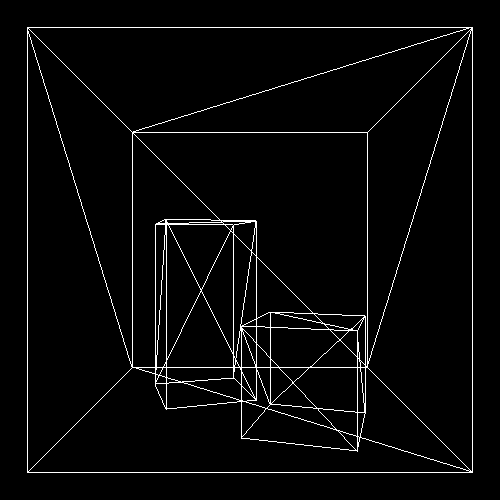
\includegraphics[width=0.45\linewidth]{screenshot1.png}
	\caption{The outlines of the polygons}
	\label{fig1}
\end{figure}
\clearpage
\subsection{Drawing Polygons}
To be able to draw the entire model, we had to go through add a lot of calculations to be able to decide which pixels was contained in each polygon. This involves first calculating the top and the bottom of the polygon as well as the leftmost and rightmost pixels.   

\begin{figure}[h!]
	\centering	
	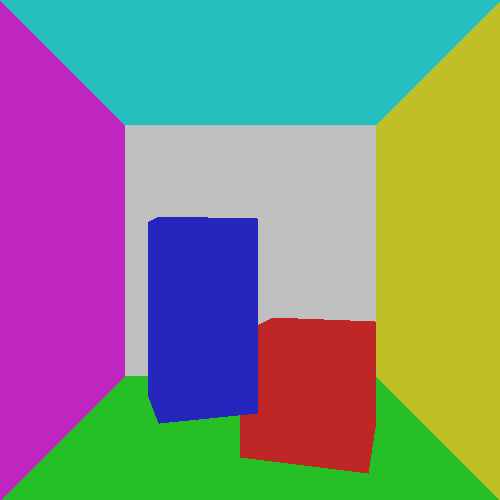
\includegraphics[width=0.45\linewidth]{screenshot15.png}
	\caption{Output of the model without using a z-buffer}
	\label{fig15}
\end{figure}

As shown in the figure \ref{fig15} the blue box is in front of the red since no z-buffer is in use.

\subsection{The z-buffer}
To be able to determine at which depth each pixel is located, a z-buffer is used. A problem with the z-buffer is that you can not use linear interpolation along the z-axis whilst using the buffer. Instead, you can linearly interpolate the z$^{-1}$ and still get a good result. Below is a print of the z-buffer:

\begin{figure}[h!]
	\centering
	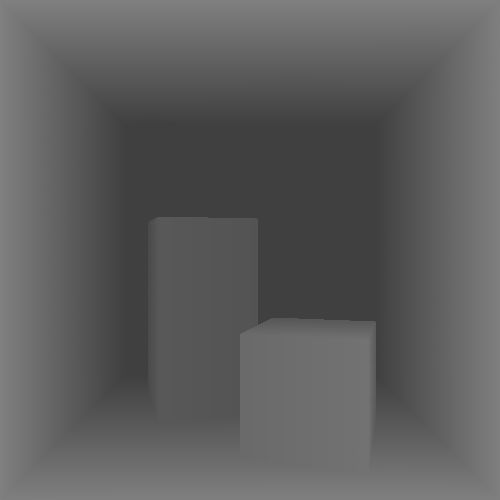
\includegraphics[width=0.45\linewidth]{screenshotz.png}
	\caption{The Z-Buffer}
	\label{figz}
\end{figure}

\subsection{Lighting}


\section{Result}
This lab was a bit more complex then the first one. We had same trouble with the comparisons of floating point number and integers eg. float == 0 is often not true due to bad precision of floating point numbers. This gave us some strange behaviors in the beginning.



-Perspective-correct interpolation. 


As can be seen above, a picture without lighting is ridiculously far from a realistic looking pictures but as soon as lighting and shadows are introduced it gets better real fast. It was fun to se the picture evolving for each completed implementation step. 

\begin{figure}[h!]
	\centering
	\begin{subfigure}[h]{0.3\linewidth}
		\centering
		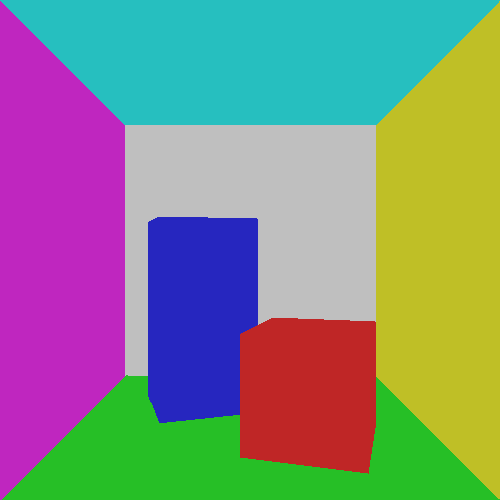
\includegraphics[width=\linewidth]{screenshot2.png}
		\caption{Facing away from light}
		\label{fig2}
	\end{subfigure}
	\begin{subfigure}[h!]{0.3\linewidth}
		\centering
		
\includegraphics[width=\linewidth]{screenshot3.png}
		\caption{With shadows}
		\label{fig3}
	\end{subfigure}
	\begin{subfigure}[h!]{0.3\linewidth}
		\centering
		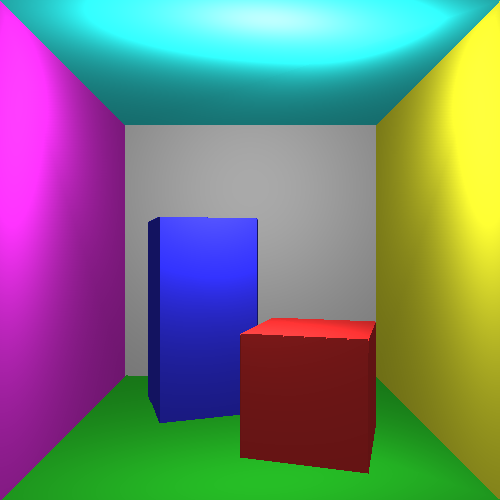
\includegraphics[width=\linewidth]{screenshot4.png}
		\caption{With shadows and colors}
		\label{fig4}
	\end{subfigure}
	\caption{Progress of the direct light model}
\end{figure}

\begin{figure}[h!]
	\centering	
	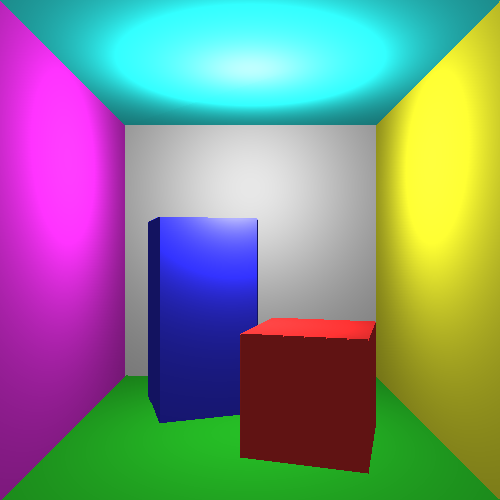
\includegraphics[width=0.45\linewidth]{screenshot5.png}
	\caption{Output from the finished program}
	\label{fig5}
\end{figure}

\begin{figure}[h!]
	\centering	
	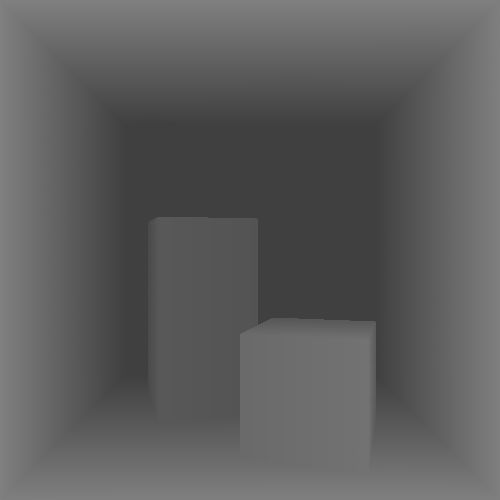
\includegraphics[width=0.45\linewidth]{screenshotz.png}
	\caption{Output from the finished program}
	\label{fig5}
\end{figure}

\begin{figure}[h!]
	\centering	
	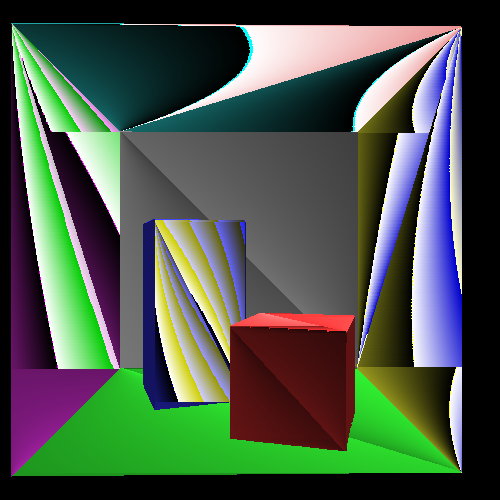
\includegraphics[width=0.45\linewidth]{fun.png}
	\caption{Output from the finished program}
	\label{fig5}
\end{figure}
\begin{figure}[h!]
	\centering	
	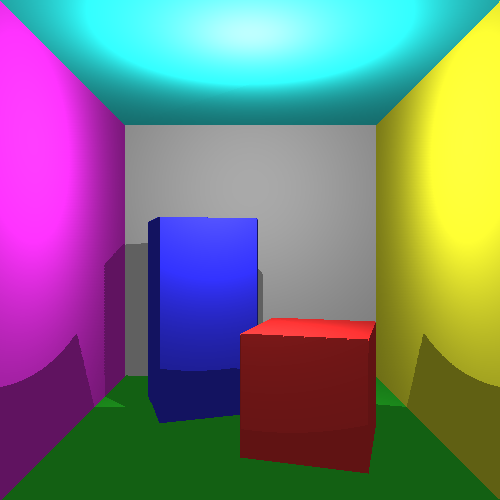
\includegraphics[width=0.45\linewidth]{shadows.png}
	\caption{Output from the finished program}
	\label{fig5}
\end{figure}

\end{document}
